\documentclass[main.tex]{subfiles}

\begin{document}
	


In order to propose an output-based controller design for the system, the matrices of equation \eqref{eq:totaldynamicslinears} are analyzed. 

Initially, it can be noticed that the main diagonal of $\bar{A}_{ocl}$, $\bar{A}_{1cl}$ and $\bar{A}_{2cl}$ have the same structure for both the inclination and the azimuth. Matrices $A_{0c}$, $A_{1c}$ and $A_{2c}$ couple the azimuth dynamics with the inclination dynamics, but this coupling is only present in terms of the inclination observer error and the integral action of the inclination observer. This fact can be used advantageously, since the inclination observer error dynamics does not depend on the azimuth dynamics. Figure \ref{fig:ISS} depicts a cascaded structure showing how the error dynamics and the observer error dynamics are interconnected.

\begin{figure}[h]\centering
	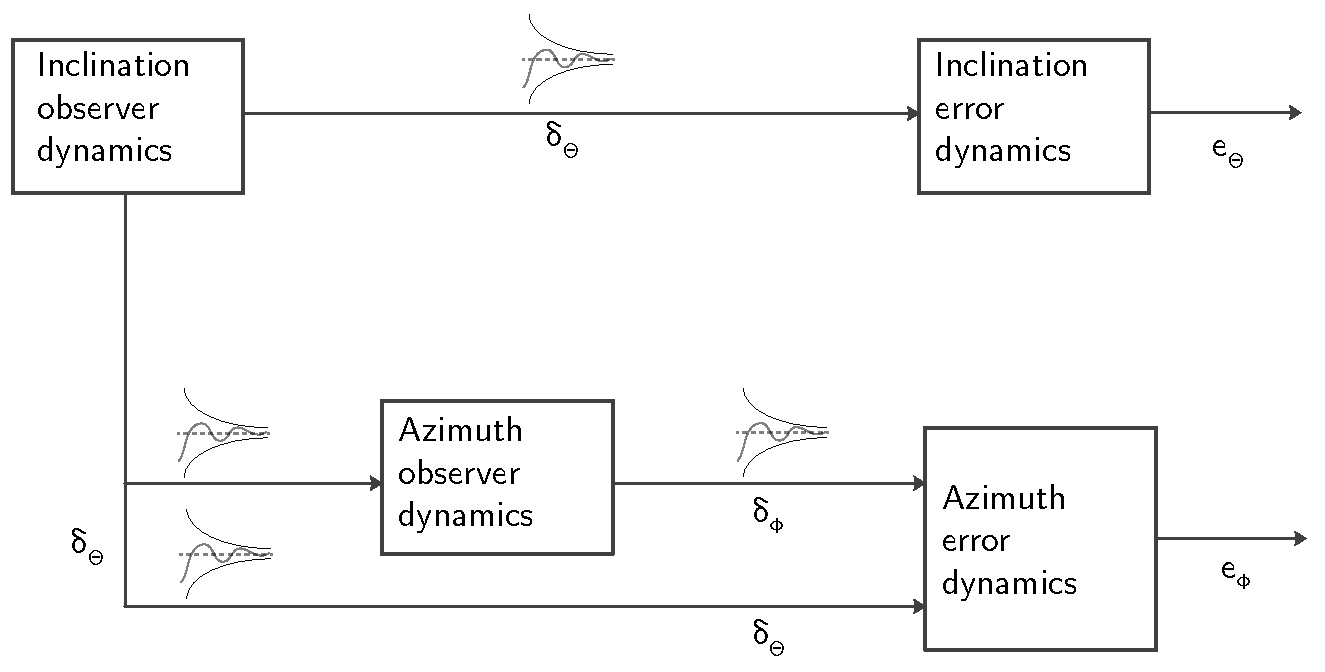
\includegraphics[width=0.5\textwidth]{ISS.pdf}
	\caption{Cascaded structure for stability of the system.
		\label{fig:ISS} }
\end{figure}

As mentioned before, the inclination dynamics are independent from the azimuth dynamics. It is important to stress this fact since this unilateral coupling is the key element for the stability analysis in this neutral bit walk case. Considering the inclination, the error and the observer error dynamics are in a series interconnection, and this interconnection is through constant ($\xi$-independent) terms, allowing to design controller and observer separately due to its linear time-invariant nature, complying with the separation principle. 

It is important to analyze the signal coming out of the inclination observer error dynamics, since it perturbs the rest of the system, as depicted in Figure \ref{fig:ISS}. As stated before, the design for the observer gain $L_\Theta$ can be done independently and this dynamics are guaranteed to be asymptotically stable if the poles of $\delta_\Theta$ are located on the left-hand side of the complex plane. On the other hand, the way this signal is interconnected with the blocks $\delta_\Phi$ and $e_\Phi$ is through $\xi$-dependent terms (namely, the "$p(\xi)$" terms). This may render controller design difficult, since this coefficients change along the trajectory, which would not allow to take an eigenvalue approach to design the azimuth observer and controller. Despite this, the $\xi$-dependent terms are entirely related to the designed reference trajectory, meaning that this terms remain bounded according to the reference trajectory. 

If then the combination of the signal coming from the $\delta_\Theta$ block and the $\xi$-dependent terms is considered, it is known that $\delta_\Theta$ is asymptotically stable (and eventually equal to zero) and that the "$p(\xi)$" terms are bounded, making the perturbation signals coming into the $\delta_\Phi$ and $e_\Phi$ blocks stable. Another remark is that there is also coupling through a $\xi$-dependent term in $\delta_\Phi$ and $e_\Phi$, related to the state $q_\Theta$, for which the same argument of it being asymptotically stable (since it corresponds to the observer integral action of the inclination, which should be stable by design) and the boundedness of its coupling term also holds.

In order to guarantee stability of the whole system, it only remains to check the internal stability of the $\delta_\Phi$ and $e_\Phi$ blocks in Figure \ref{fig:ISS}. Considering that the perturbation signal going into these blocks is asymptotically stable, the stability of the error and observer error dynamics can be analysed without considering them. This leads to the same series interconnection from $\delta_\Phi$ to $e_\Phi$, allowing to design once again, controller and observer gains separately, without compromising stability of the whole system. An important observation as well, is that the linearized system stability is independent from the trajectory, as this only influences the interconnection terms.

After this analysis, it can be concluded that the controller synthesis of gains $K_i$ and $L_i$ can be done using an eigenvalue approach as in \cite{Kremers2013} and \cite{Monsieurs2015}, for the following isolated system dynamics:

\begin{align}
	\begin{bmatrix}
		e_\Theta'(\xi) \\
		\Delta \bar{\Gamma}_\Theta^{*'}(\xi) \\
		\Delta z_{1\Theta}'(\xi) \\
		\Delta z_{2\Theta}'(\xi) \\
	\end{bmatrix} =& 
	\begin{bmatrix}[cccc]
	A_0 & 0 & 0 & B\\
	%
	0 & -b_0 & 0 & -b_1\\
	\zeta \begin{bmatrix}k_{1\Theta} , 0 , 0\end{bmatrix} & 0 & 0 & 0\\
	%
	\gamma K_\Theta & 0 & \gamma & -\gamma
	\end{bmatrix}
	\begin{bmatrix}
	e_\Theta(\xi) \\
	\Delta \bar{\Gamma}_\Theta^{*}(\xi) \\
	\Delta z_{1\Theta}(\xi) \\
	\Delta z_{2\Theta}(\xi) \\
	\end{bmatrix} + 
	\begin{bmatrix}[cccc]
	A_1 & 0 & 0 & 0\\
	%
	0 & 0 & 0 & 0\\
	0 & 0 & 0 & 0\\
	%
	0 & 0 & 0 & 0 
	\end{bmatrix}
	\begin{bmatrix}
	e_\Theta(\xi_1) \\
	\Delta \bar{\Gamma}_\Theta^{*}(\xi_1) \\
	\Delta z_{1\Theta}(\xi_1) \\
	\Delta z_{2\Theta}(\xi_1) \\
	\end{bmatrix} \nonumber\\
	&+ 
	\begin{bmatrix}[cccc]
	A_2 & 0 & 0 & 0\\
	%
	0 & 0 & 0 & 0\\
	0 & 0 & 0 & 0\\
	%
	0 & 0 & 0 & 0 
	\end{bmatrix}
	\begin{bmatrix}
	e_\Theta(\xi_2) \\
	\Delta \bar{\Gamma}_\Theta^{*}(\xi_2) \\
	\Delta z_{1\Theta}(\xi_2) \\
	\Delta z_{2\Theta}(\xi_2) \\
	\end{bmatrix} \label{eq:SynthesisConInc}\\
	%
	%
	%
	\nonumber\\
	\begin{bmatrix}
	e_\Phi'(\xi) \\
	\Delta \Gamma_\Phi^{*'}(\xi) \\
	z_{1\Phi}'(\xi) \\
	z_{2\Phi}'(\xi) \\
	\end{bmatrix} =& 
	\begin{bmatrix}[cccc]
	A_0 & 0 & 0 & B\\
	%
	0 & -b_0 & 0 & -b_1\\
	\zeta \begin{bmatrix}k_{1\Phi} , 0 , 0\end{bmatrix} & 0 & 0 & 0\\
	%
	\gamma K_\Phi & 0 & \gamma & -\gamma
	\end{bmatrix}
	\begin{bmatrix}
	e_\Phi(\xi) \\
	\Delta \Gamma_\Phi^{*}(\xi) \\
	z_{1\Phi}(\xi) \\
	z_{2\Phi}(\xi) \\
	\end{bmatrix} + 
	\begin{bmatrix}[cccc]
	A_1 & 0 & 0 & 0\\
	%
	0 & 0 & 0 & 0\\
	0 & 0 & 0 & 0\\
	%
	0 & 0 & 0 & 0 
	\end{bmatrix}
	\begin{bmatrix}
	e_\Phi(\xi_1) \\
	\Delta \Gamma_\Phi^{*}(\xi_1) \\
	z_{1\Phi}(\xi_1) \\
	z_{2\Phi}(\xi_1) \\
	\end{bmatrix} \nonumber\\
	&+ 
	\begin{bmatrix}[cccc]
	A_2 & 0 & 0 & 0\\
	%
	0 & 0 & 0 & 0\\
	0 & 0 & 0 & 0\\
	%
	0 & 0 & 0 & 0 
	\end{bmatrix}
	\begin{bmatrix}
	e_\Phi(\xi_2) \\
	\Delta \Gamma_\Phi^{*}(\xi_2) \\
	z_{1\Phi}(\xi_2) \\
	z_{2\Phi}(\xi_2) \\
	\end{bmatrix} \label{eq:SynthesisConAzi}\\
	%
	%
	%
	\nonumber\\
	\begin{bmatrix}
	\delta_\Theta  '(\xi) \\
	\Delta q_\Theta'(\xi)
	\end{bmatrix} =&
	\begin{bmatrix}[cc]
	A_0 - L_\Theta C_\Theta & -B\\ 
	%
	\zeta \begin{bmatrix}l_{1\Theta} , l_{2\Theta}	\end{bmatrix} C_\Theta & 0
	\end{bmatrix}
	\begin{bmatrix}
	\delta_\Theta (\xi)\\
	\Delta q_\Theta (\xi)
	\end{bmatrix} + 
	\begin{bmatrix}[cc]
	A_1 & 0\\ 
	%
	0 & 0
	\end{bmatrix}
	\begin{bmatrix}
	\delta_\Theta (\xi_1)\\
	\Delta q_\Theta (\xi_1)
	\end{bmatrix} + 
	\begin{bmatrix}[cc]
	A_2 & 0\\ 
	%
	0 & 0
	\end{bmatrix}
	\begin{bmatrix}
	\delta_\Theta (\xi_2)\\
	\Delta q_\Theta (\xi_2)
	\end{bmatrix} \label{eq:SynthesisObsInc}\\
    	%
    	%
    	%
    	\nonumber \\
    	\begin{bmatrix}
    	\delta_\Phi  '(\xi) \\
    	q_\Phi'(\xi)
    	\end{bmatrix} =&
    	\begin{bmatrix}[cc]
    	A_0 - L_\Phi C_\Phi & -B\\ 
    	%
    	\zeta \begin{bmatrix}l_{1\Phi} , l_{2\Phi}	\end{bmatrix} C_\Phi & 0
    	\end{bmatrix}
    	\begin{bmatrix}
    	\delta_\Phi (\xi)\\
    	q_\Phi (\xi)
    	\end{bmatrix} + 
    	\begin{bmatrix}[cc]
    	A_1 & 0\\ 
    	%
    	0 & 0
    	\end{bmatrix}
    	\begin{bmatrix}
    	\delta_\Phi (\xi_1)\\
    	q_\Phi (\xi_1)
    	\end{bmatrix} + 
    	\begin{bmatrix}[cc]
    	A_2 & 0\\ 
    	%
    	0 & 0
    	\end{bmatrix}
    	\begin{bmatrix}
    	\delta_\Phi (\xi_2)\\
    	q_\Phi (\xi_2)
    	\end{bmatrix} \label{eq:SynthesisObsAzi}
\end{align}

Stability can be achieved if gains $K_i$ and $L_i$ are chosen in such way that the poles of \eqref{eq:SynthesisConInc}, \eqref{eq:SynthesisConAzi}, \eqref{eq:SynthesisObsInc} and \eqref{eq:SynthesisObsAzi} are on the left half of the complex plane. Despite that stability can be ensure, the performance of the system could not be adequate, since the initial error in estimation could cause a high level of transient oscillations (borehole spiraling) and if it is above certain limit, this could generate a steady state error in the final response of the azimuth dynamics, since the system is performing far away from the linearization.

In order to cope with this initial estimation error, it is proposed to use the available measurements of the BHA orientation close to the bit as initial value for the observer dynamics. These measurements are given by output equations in \eqref{eq:output1} and \eqref{eq:output2}.

\subsection{Controller and observer gain design}

Although the structure of the controller has already been decided, it remains to choose the values of the controller, observer, integral-action and low-pass filter gains. The stability of the system is guaranteed as long as the closed-loop poles are located on the left-hand side of the imaginary axis in the complex plane. In other words, for the system to be stable, the following conditions have to be met (for corresponding isolated systems \eqref{eq:SynthesisConInc}, \eqref{eq:SynthesisConAzi}, \eqref{eq:SynthesisObsInc} and \eqref{eq:SynthesisObsAzi}):

\begin{align}
	\max_{j\in[1,2,...,\infty]} \{\Re(\lambda_{jK\Theta}(K_{\Theta},\zeta,\gamma)) \} < 0,
	\label{eq:condition1} \\
	\max_{j\in[1,2,...,\infty]} \{\Re(\lambda_{jK\Phi}(K_{\Phi},\zeta,\gamma)) \} < 0,
	\label{eq:condition2} \\
	\max_{j\in[1,2,...,\infty]} \{\Re(\lambda_{jL\Theta}(L_{\Theta},\zeta)) \} < 0,
	\label{eq:condition3} \\
	\max_{j\in[1,2,...,\infty]} \{\Re(\lambda_{jL\Phi}(L_{\Phi},\zeta)) \} < 0,
	\label{eq:condition4}
\end{align}

where $\lambda_{jKi}(K_{i},\zeta,\gamma)$ and $\lambda_{jLi}(L_{i},\zeta)$ for $i = \Theta, \Phi$ represent closed-loop pole $j$ of the isolated systems corresponding to the controller and observer dynamics, respectively. Furthermore, the settling time of the isolated system decreases as the poles are located further to the left. In other to obtain specific values for the controller and observer gains, based on the conditions given by \eqref{eq:condition1}, \eqref{eq:condition2}, \eqref{eq:condition3} and \eqref{eq:condition4}we can formulate an optimization problem consisting on minimizing the following objective functions:

\begin{align}
\varLambda_1 &= \max_{j\in[1,2,...,\infty]} \{\Re(\lambda_{jK\Theta}(K_{\Theta},\zeta,\gamma)) \},
\label{eq:op1} \\
\varLambda_2  &= \max_{j\in[1,2,...,\infty]} \{\Re(\lambda_{jK\Phi}(K_{\Phi},\zeta,\gamma)) \} ,
\label{eq:op2} \\
\varLambda_3 &= \max_{j\in[1,2,...,\infty]} \{\Re(\lambda_{jL\Theta}(L_{\Theta},\zeta)) \},
\label{eq:op3} \\
\varLambda_4 &= \max_{j\in[1,2,...,\infty]} \{\Re(\lambda_{jL\Phi}(L_{\Phi},\zeta)) \},
\label{eq:op4}
\end{align}

corresponding to isolated systems \eqref{eq:SynthesisConInc}, \eqref{eq:SynthesisConAzi}, \eqref{eq:SynthesisObsInc} and \eqref{eq:SynthesisObsAzi}, respectively. This non-smooth optimization problem can be solved using a gradient-sampling algorithm \cite{Kremers2013}. This algorithm can be implemented via the Matlab toolbox \cite{Michiels:2007:SST:1355294}, which also allows to choose the location of the real part of the right-most pole. Despite this, the objective functions proposed can be computationally expensive. In order to reduce the effort, the gains of the integral action $\zeta$ and the low-pass filter $\gamma$ are fixed for each iteration. This can be done since the control objectives that these gains pursue are on a different "length" scale as the control objectives that the state-feedback and observer gains \cite{Monsieurs2015}. The selection of these gains will be done in an iterative process until the desired performance is reached.

It has to be kept in mind that, since the inclination observer dynamics have to converge faster than the rest of the dynamics of the system, the location of its right-most pole has to be chosen further than for the rest of the rest of the dynamics of the system, this will be explained in the next section.


\subsection{Controller synthesis}

In order to propose the values for the right-most poles for the optimization problem to compute the controller and observer gains, a time ('length') scale for the convergence of $\delta_i$ and $e_i$ based on the cascaded structure of Figure \ref{fig:ISS} is introduced. The determining dynamics of the cascaded structure are given by the $\delta_\Theta$ block. Because of this, it has been decided to set this as $fast$ converging dynamics. As long as the rest of the elements in the structure have a slower convergence, the inclination observer will not lead to large transients in the other dynamics (regarding $\delta_\Phi$, $e_\Theta$ and $e_\Phi$) which would invalidate the assumptions motivating the stability analysis based on linearization. On the other hand, $\delta_\Phi$ has to be faster than $e_\Phi$, so it is placed in a $medium$ scale. For the error dynamics $e_\Theta$ and $e_\Phi$, the choice can be made to set $e_\Theta$ in the same $medium$ time scale as $\delta_\Phi$ and to set $e_\Phi$ in a $slow$ time scale (since inclination does not depend on the azimuth). It has been decided to keep $e_\Theta$ and $e_\Phi$ on the same $slow$ time scale to have a similar behavior for both $\Theta$ and $\Phi$.

Table \ref{table:controllervalues} shows the values chosen for the low-pass filter and integral part fixed for the optimization, as well as the value of the real part of the right-most pole and its corresponding computed feedback gains.

\begin{table}[h]
\centering
\caption{Parameters for controller gains.}
\label{table:controllervalues}
\begin{tabular}{|l|l|l|l|l|}
\hline
Gain & Objective function right-most pole location & Feedback values & $\gamma$ & $\zeta$ \\ \hline
$e_\Theta$ & -0.6 & $K_\Theta = \begin{bmatrix} -6310 & -2571 & 1288 \end{bmatrix}$ & 0.8 & 0.5\\ \hline
$\delta_\Theta$ & -0.9 & $L_\Theta = \begin{bmatrix} 1014 & 3299 \\ 0 & 0 \\ 0 & 0\end{bmatrix}$ & 0 & 0.5\\ \hline
$e_\Phi$   & -0.6 & $K_\Phi = \begin{bmatrix} -7058 & -72.1 & 1021 \end{bmatrix}$ & 0.8 & 0.3\\ \hline
$\delta_\Phi$   & -0.7 & $L_\Phi = \begin{bmatrix} -48.5 & 2555 \\ 0 & 0 \\ 0 & 0\end{bmatrix}$ & 0 & 0.3 \\\hline
\end{tabular}
\end{table}

The most critical values to be designed are the ones corresponding to the inclination observer error $\delta_\Theta$, since all of the dynamics are in a series interconnection with its states. It can be seen that the real part of the right-most pole is chosen to be the furthest from the imaginary axis, in order to have a faster convergence. It has to be considered as well, that if the poles are pushed too much to the left, this could result in high observer gains, which could potentially amplify the effect of disturbances such as noise or model uncertainty. The integrator value is chosen to be the same as the one for the error dynamics, since it is also counteracting the effect of gravity related terms. It has been chosen to not implement a low-pass filter in both observers, since its function is to avoid fast changes in the response, which is not a problem in the estimation error. The low-pass filter gains are kept the same for both the inclination and azimuth tracking error dynamics. As for the integral part of the azimuth error $e_\Phi$ and the observer error $\delta_\Phi$, despite the fact that there are no gravity terms affecting the these dynamics, the initial error of $\delta_\Theta$ could act as a disturbance for a short period of time. This could be analogous to an impulse-like disturbance, which can be effectively rejected by implementing integral action. This is implemented in both the controller an observer of the azimuth, although with different gains, since the disturbance to be rejected is of a different type. 

Figure \ref{fig:ClosedLoopPolesNeutral} shows the union of the closed-loop poles of the isolated systems \eqref{eq:SynthesisConInc}, \eqref{eq:SynthesisConAzi}, \eqref{eq:SynthesisObsInc} and \eqref{eq:SynthesisObsAzi} after implementing the controller gains of table \ref{table:controllervalues}. The right-most pole (poles at the origin are not considered since they are introduced by the state description) is at -0.6195, which is above the chosen maximum value for the right-most poles of the error dynamics.

\begin{figure}[h]\centering
	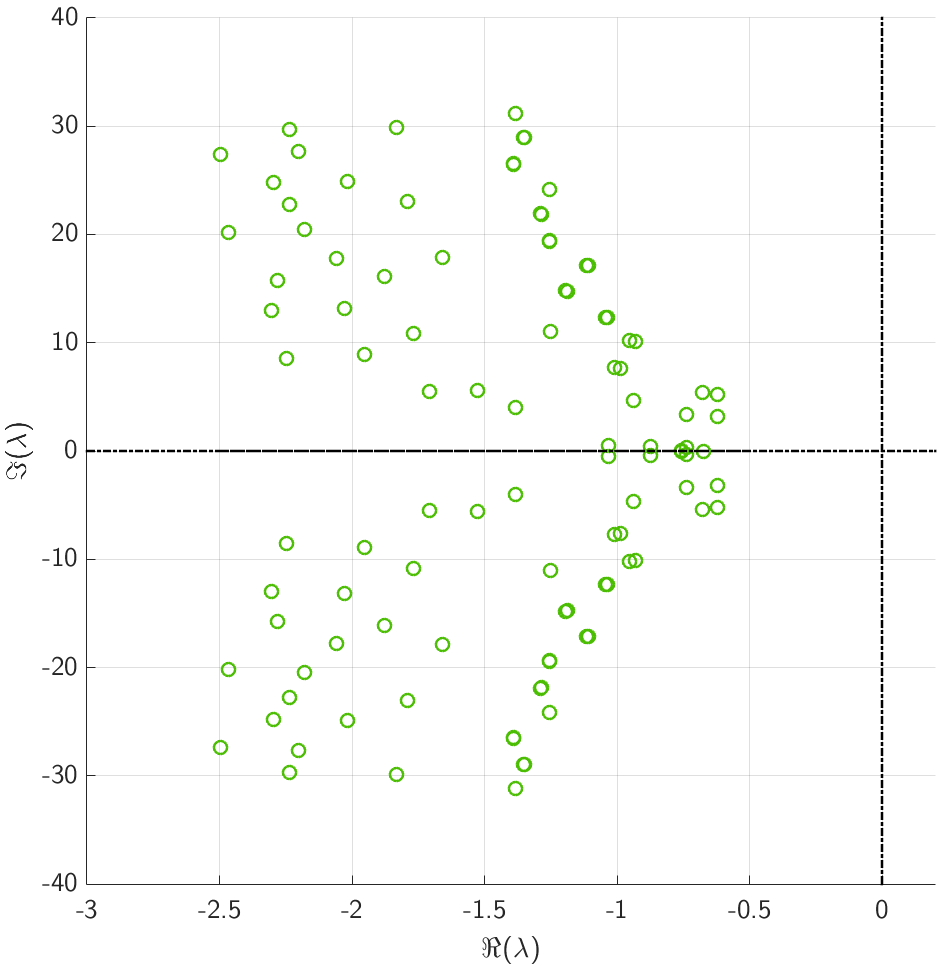
\includegraphics[width=0.5\textwidth]{ClosedLoopPolesNeutral.png}
	\caption{Closed-loop poles for the neutral bit walk system for $\eta \Pi = 0.261$.
		\label{fig:ClosedLoopPolesNeutral} }
\end{figure}


To implement the controller the desired trajectory to follow is the same as in \cite{Monsieurs2015}. The controller will be tested for several initial conditions, since its behavior could be sensitive to initial errors in the observer. The first measurement of the sensor is being taken into account to improve the transient response. Figure \ref{fig:Resoponse} shows the inclination and azimuth response for each set of initial conditions.

\begin{figure}[H]\centering
	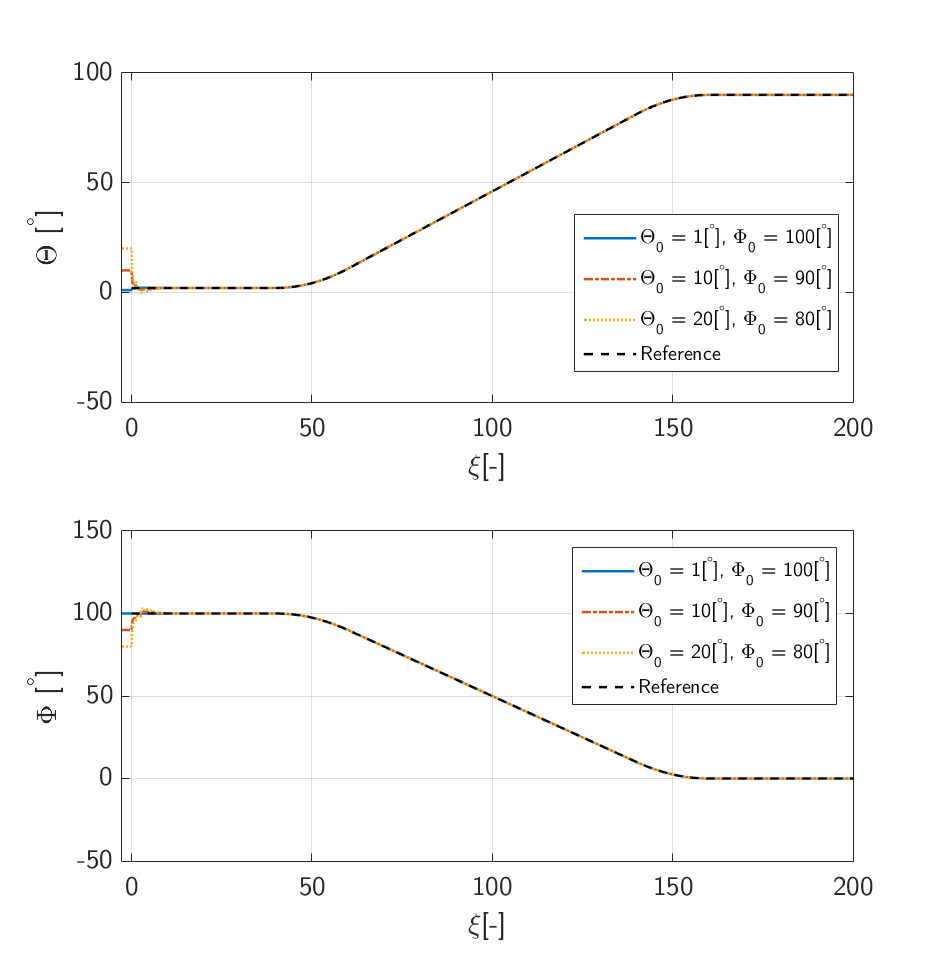
\includegraphics[height=3.5in]{Response.png}
	\caption{Inclination and azimuth responses of the system.
		\label{fig:Resoponse} }
\end{figure}


Despite the fact that the initial condition does affect the transient at the beginning of the response, the controller is able to track the trajectory close to the reference. It also has to be considered the influence of the initial condition in the applied RSS force, this is depicted in Figure \ref{fig:RSSForces}.

\begin{figure}[H]\centering
	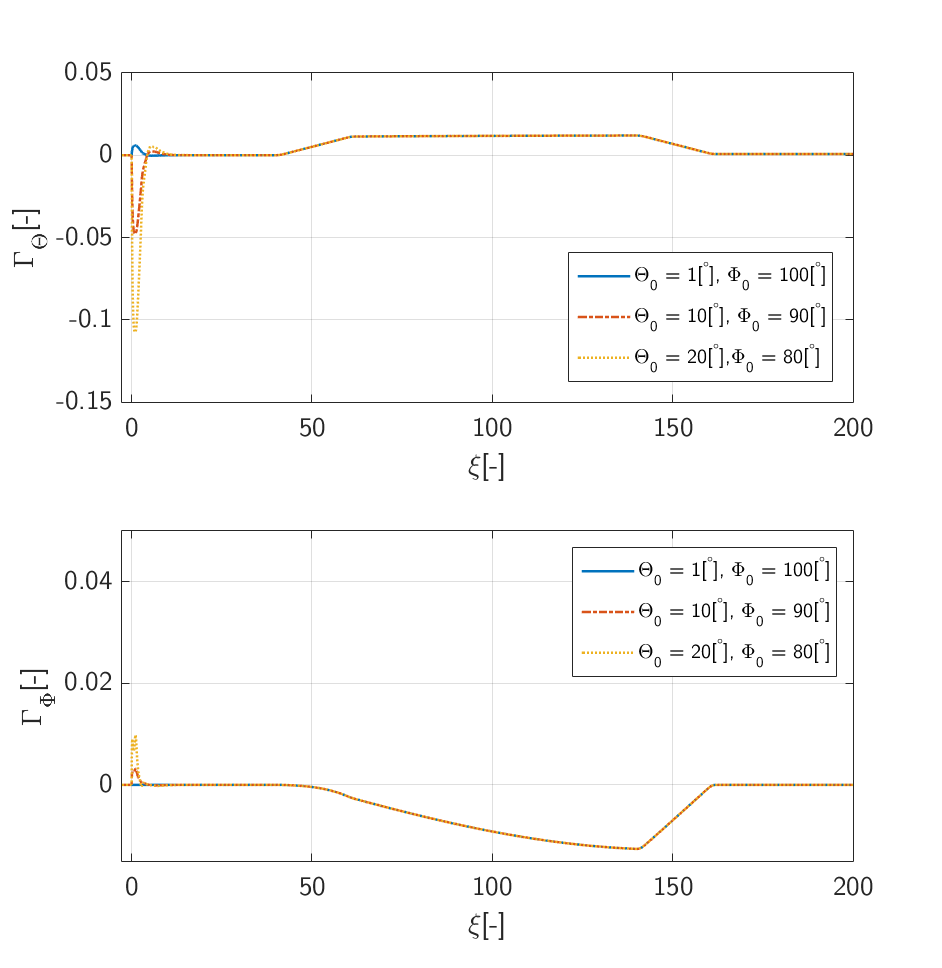
\includegraphics[height=3.5in]{RSSInputs.png}
	\caption{RSS Forces applied to the system.
		\label{fig:RSSForces} }
\end{figure}

The influence of the initial condition is clearly seen as well when the RSS begins to be applied, for both the inclination and the azimuth. This has to do with the fact that although the initial condition is taken from the measurement, as you start further away from the reference, the RSS has to apply more force in order to compensate for that initial error. Finally, the system and observer errors are shown in Figures \ref{fig:ErrorNeutral} and \ref{fig:ObserverErrors}, up to $\xi = 25$ since the error already converged to zero. 


\begin{figure}[H]\centering
	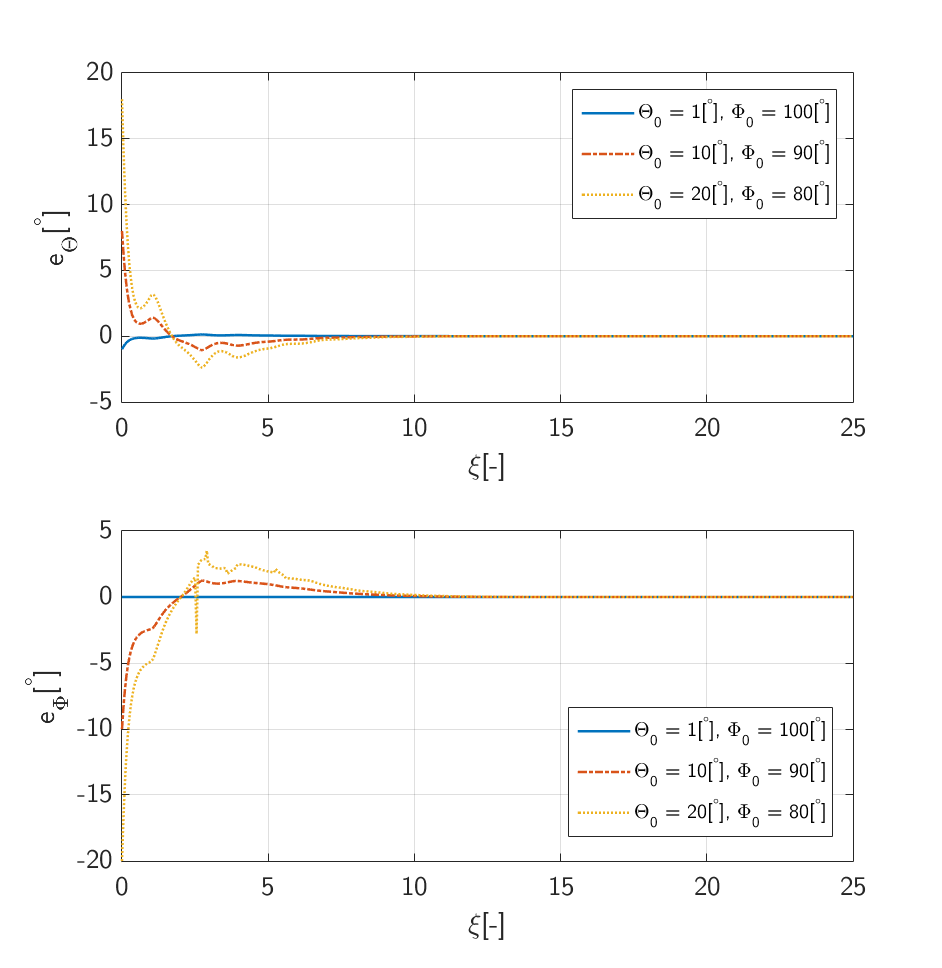
\includegraphics[height=3.5in]{ErrorsNeutral.png}
	\caption{Errors for different initial conditions.
		\label{fig:ErrorNeutral} }
\end{figure}

\begin{figure}[H]\centering
	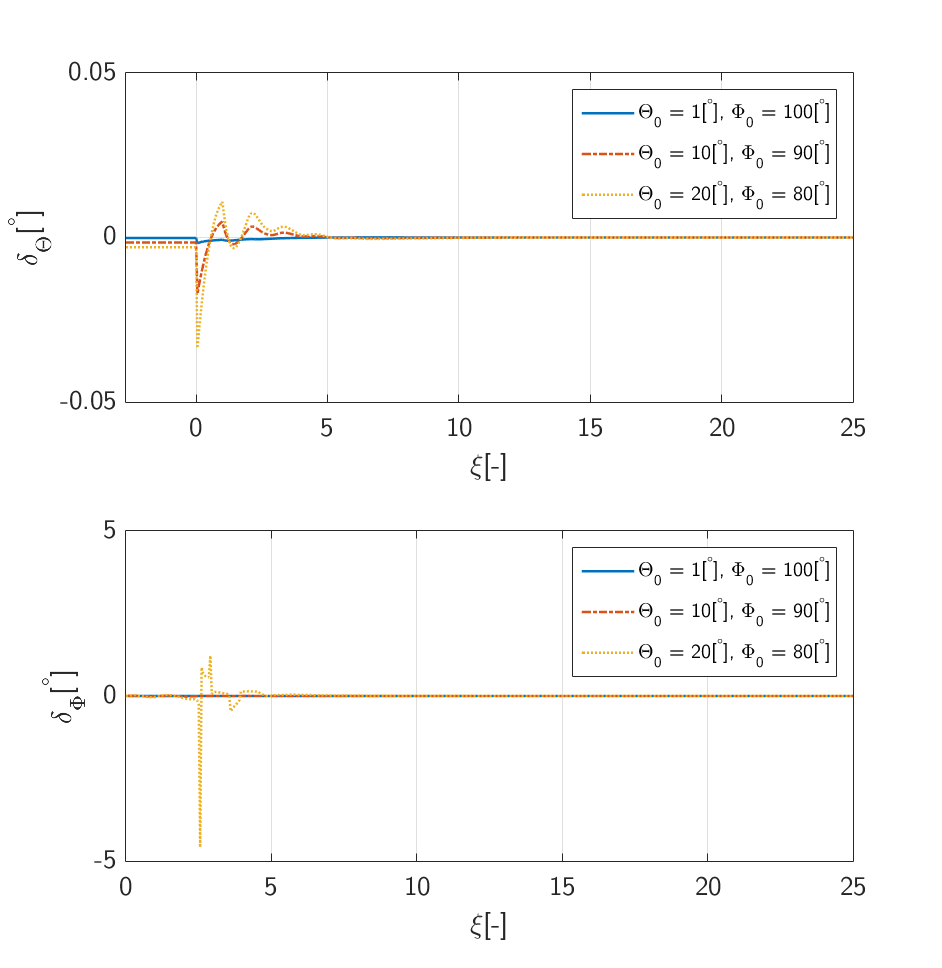
\includegraphics[height=3.5in]{ObserverErrors.png}
	\caption{Observer errors for different initial conditions.
		\label{fig:ObserverErrors} }
\end{figure}

The error for both the inclination and the azimuth reaches the value of zero at approximately $\xi = 10$, this result complies with a fast enough response in order to drill a complex borehole geometry. The behavior of the observer is as expected in the case of the inclination, since the initial condition is further from the reference, and the difference between the measurement and the value of $\Theta$ starts increasing as the absolute value of $\Theta_0$ increases, if we consider Equation \eqref{eq:output12}. 

On the other hand, the observer error of the azimuth shows a particular behavior. It can be seen, that in the case of the initial condition $\Theta_0 = 20 [^{\circ}]$ and $\Phi_0 = 80[^{\circ}]$, the error is much bigger in comparison with the other two sets of initial conditions. This could be explained, since the system was linearized to work around $e_i = 0$ and $\delta_i = 0$, and the nonlinear terms were all related to the difference between $\Theta$ and $\check{\Theta}$. If there is a big enough difference between this two variables, the linearized system will no longer be valid and this could generate estimation errors. Furthermore, besides having to deal with its own initial estimation error, the error in $\delta_\Theta$ also affects the azimuth observer until it reaches zero as shown in the nonlinear dynamic equations \eqref{eq:totaldynamics}.



\end{document}

